\begin{Exercise}[title={Stack},difficulty=5]
\label{ex:stack}

\begin{wrapfigure}{l}{30mm}
\begin{center}
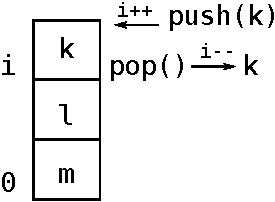
\includegraphics[scale=0.50]{fig/stack.pdf}
\end{center}
\end{wrapfigure}

\Question \label{ex:stack q1} Create a simple stack which can hold a
fixed amount of \key{int}s. It does not have to grow beyond this limit.
Define both a \func{push} -- put something on the stack -- and a \func{pop} 
-- retrieve something fro the stack -- function. The stack must be
last in, first out (LIFO).

\Question \label{ex:stack q2} Bonus. Write a \func{String} method which 
converts the stack to a string. This way you can print the stack using:
\lstinline{fmt.Printf("My stack %v\n", stack)}. This may aid in
debugging.
\end{Exercise}

\begin{Answer}

\Question First we define a new type that represents a stack; we need an
array (to hold the keys) and an index, which points to the last element.
Our small stack only holds 10 elements.

\begin{lstlisting}
type stack struct { |\coderemark{this type is not exported}|
    i    int 
    data [10]int
}
\end{lstlisting}

In Go data passed to functions is \emph{passed-by-value} meaning a copy
is created and given to the function.  First example to show

\Question While this was a bonus question, having the ability to print
the stack was very valuable when writing the code for this exercise.
According to the Go documentation \lstinline{fmt.Printf("%v")} can
print any value (\%v) that satisfies the \func{Stringer} interface.
For this to work we only need to define a \func{String()} function for
our type:
\begin{lstlisting}
func (s *stack) String() string {
	var str string
	for i := 0; i <= s.i; i++ {
		str = str + "[" +
		strconv.Itoa(i) + ":" + strconv.Itoa(s.data[i]) + "]"
	}
	return str
}
\end{lstlisting}
\end{Answer}
